\documentclass{../lista}

\begin{document}
	\cabecalho{5}{\red{Gabarito}}{Sistema Solar e História}{Iago Mendes}

	\begin{questao}{1 ponto) (0,2 cada acerto}
		Coloque o nome do astro respectivo às seguintes descrições:

		\begin{center} \begin{tabular}{|M{0.2\textwidth}|M{0.65\textwidth}|}
			\hline
			\red{Mercúrio} & Possui uma amplitude térmica altíssima, variando de $427^{\circ}C$ até $-137^{\circ}C$. Sua superfície se assemelha com a da Lua. Leva cerca de 59 dias para completar uma volta em torno de si e 88 dias para realizar uma revolução completa em torno do Sol. \\ \hline
			\red{Vênus} & Astro com maior temperatura do Sistema Solar devido ao efeito estufa de sua atmosfera. Pode ser visto no céu noturno em certas épocas do ano (sempre próximo ao Sol). Seu dia é mais longo do que seu ano. \\ \hline
			\red{Titã} & Um dos satélites naturais mais famosos no Sistema Solar, sendo o segundo maior. É o único astro -- além da Terra -- onde já foram encontradas evidências concretas da existência de corpos líquidos estáveis na superfície. Foi descoberto em 1655 pelo astrônomo Christiaan Huygens. \\ \hline
			\red{Saturno} & Astro com densidade inferior a da água. Foi estudado pela missão Cassini–Huygens. É o último planeta facilmente vísivel a olho nu da Terra e o que possui o maior número de satélites naturais encontrados. Seu anel é feito de gelo. \\ \hline
			\red{Urano} & Possui coloração azulada devido à existência de gás metano em sua atmosfera. Seus movimentos são curiosos, pois, além de ser um dos 2 planetas que rotacionam de Leste para Oeste, possui seu eixo de rotação ``deitado" em relação ao plano de translação. Possui um anel constituído por rochas.\\ \hline
		\end{tabular} \end{center}
	\end{questao}

	\begin{questao}{1 ponto) (0,2 cada acerto}
		Coloque o nome do astro respectivo às seguintes descrições:

		\begin{center} \begin{tabular}{|M{0.2\textwidth}|M{0.65\textwidth}|}
			\hline
			\red{Júpiter} & Possui faixas brancas e marrons em sua atmosfera, além de uma tempestade que gera o que chamamos de \textit{A Grande Mancha Vermelha}. Seu anel é rochoso e seus satélites naturais mais famosos foram estudados por \textit{Galileo Galilei}. \\ \hline
			\red{Marte} & Lugar do \textit{Monte Olimpo} (maior vulcão do Sistema Solar). Possui 2 satélites naturais: Phobos e Deimos. Está a uma distância de aproximadamente $1,5 \, UA$ do Sol. \\ \hline
			\red{Cometa Halley} & Possui afélio no \textit{Cinturão de Kuiper} e periélio a cerca de $0,6 \, UA$ do Sol. Composto majoritariamente por rochas, poeira, e gases congelados. Seu período orbital é aproximadamente $76$ anos. \\ \hline
			\red{Ganimedes} & Descoberto por \textit{Galileo Galilei} em 1610. É o maior e mais massivo satélite natural do Sistema Solar. Pode ser observado próximo ao planeta em torno de qual orbita, estando algumas vezes alinhado com outros 3 astros.  \\ \hline
			\red{Plutão} & Suas primeiras imagens de qualidade foram tiradas pela sonda \textit{New Horizons} em 2015. É um objeto transnetuniano, pertencendo ao \textit{Cinturão de Kuiper}. Em 2006, devido a uma redefinição feita pela \textit{IAU}, sua classificação foi alterada. \\ \hline
		\end{tabular} \end{center}
	\end{questao}

	\begin{questao}{1 ponto) (0,25 cada acerto}
		Marque a segunda coluna em relação à primeira, indicando a classificação correta de cada astro.
		\begin{multicols}{2}
			\vfill\null \vfill\null
			\begin{flushleft}
				(1) Planeta anão \\
				(2) Satélite natural \\
				(3) Cometa de curto período \\
				(4) Cometa de longo período
			\end{flushleft}
			\vfill\null \vfill\null
			\columnbreak

			\begin{alternativas}
				\alternativaMarcada[$\red{4}$] Astro popularmente conhecido como Neowise, mas com nome oficial C/2020 F3. Foi descoberto em 2020. Está localizado na Nuvem de Oort. Possui um período orbital de aproximadamente $6.766$ anos.
				\alternativaMarcada[$\red{1}$] Astro chamado Ceres. Foi descoberto em 1801. Está localizado no Cinturão de Asteroides. Possui um período orbital de aproximadamente $5$ anos.
				\alternativaMarcada[$\red{3}$] Astro popurlamente conhecido como Halley, mas com nome oficial 1P/Halley. Foi descoberto em 1758. Está localizado no Cinturão de Kuiper. Possui um período orbital de aproximadamente $76$ anos.
				\alternativaMarcada[$\red{2}$] Astro chamado Encélados. Foi descoberto em 1789. Está localizado na faixa de planetas gasosos. Possui um período orbital de aproximadamente 33 horas.
			\end{alternativas}
		\end{multicols}
	\end{questao}

	\begin{questao}{1 ponto) (0,3 cada acerto + 0,1 se acertar todos}
		Marque a segunda coluna em relação à primeira, indicando qual astrônomo foi responsável pelos feitos descritos.
		\begin{multicols}{2}
			\vfill\null \vfill\null
			\begin{flushleft}
				(1) Galileo Galilei \\
				(2) Sir Isaac Newton \\
				(3) Johannes Kepler
			\end{flushleft}
			\vfill\null \vfill\null
			\columnbreak
			\begin{alternativas}
				\alternativaMarcada[$\red{3}$] Nasceu em 1571. Criou 3 leis que tinham como objetivo descrever o movimento dos planetas. Desenvolveu um tipo de telescópio refrator, em que as lentes objetiva e ocular são convergentes.
				\alternativaMarcada[$\red{1}$] Nasceu em 1564. Desenvolveu um tipo de telescópio refrator, em que as lentes objetiva e ocular são convergente e divergente, respectivamente. Descobriu os 4 satélites naturais principais do maior planeta do Sistema Solar.
				\alternativaMarcada[$\red{2}$] Nasceu em 1643. Criou 3 leis que são usadas como base da Dinâmica, divisão da Mecânica. Desenvolveu um tipo de telescópio refletor, em que os espelhos principal e secundário são côncavo e plano, respectivamente.
			\end{alternativas}
		\end{multicols}
	\end{questao}

	\begin{questao}{1 ponto}
		Por muitos anos, houve o debate sobre qual modelo seria o mais adequado para descrever o nosso sistema solar: modelo geocêntrico ou heliocêntrico. Para responder às perguntas desta questão, considere os esquemas seguintes, os quais mostram o funcionamento básico de cada modelo:
		\begin{figure}[H] \label{img:geocentrico}
	\centering
	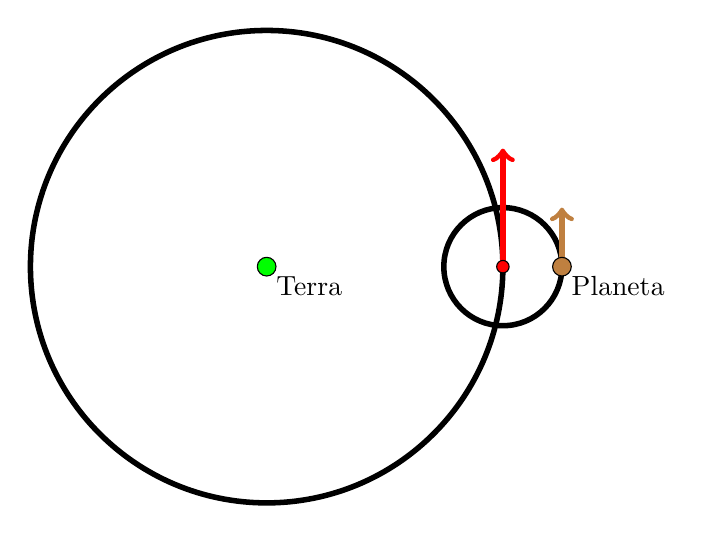
\begin{tikzpicture}[scale=0.75]
	[
		line cap=round,
		line join=round,
		>=triangle 45,
		x=1cm,
		y=1cm
	]
		\draw [line width=2pt] (0,0) circle (4cm);
		\draw [line width=2pt] (4,0) circle (1cm);
		\draw [->,line width=2pt,color=brown] (5,0) -- (5,1);
		\draw [->,line width=2pt,color=red] (4,0) -- (4,2);
		\draw (0,0) node[anchor=north west] {Terra};
		\draw (5,0) node[anchor=north west] {Planeta};
		\begin{scriptsize}
			\draw [fill=green] (0,0) circle (4.5pt);
			\draw [fill=red] (4,0) circle (3pt);
			\draw [fill=brown] (5,0) circle (4.5pt);
		\end{scriptsize}
	\end{tikzpicture}
	\captionsetup{labelformat=empty}
	\caption{\textbf{Esquema 1:} Modelo geocêntrico}
\end{figure}
		\begin{figure}[H] \label{img:heliocentrico}
	\centering
	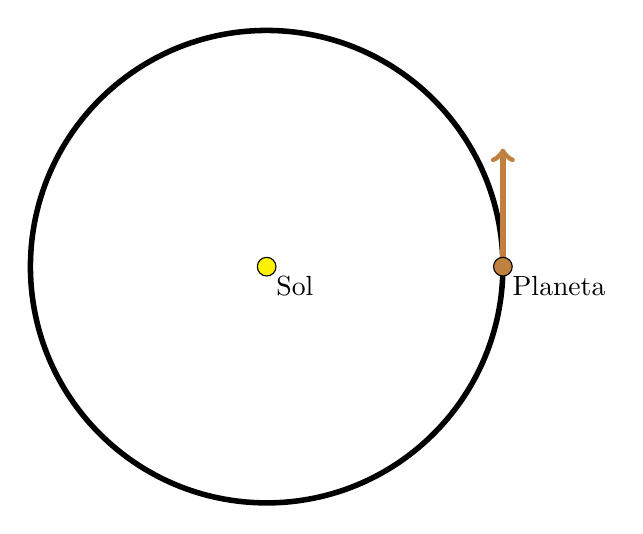
\begin{tikzpicture}[scale=0.75]
	[
		line cap=round,
		line join=round,
		>=triangle 45,
		x=1cm,
		y=1cm
	]
		\draw [line width=2pt] (0,0) circle (4cm);
		\draw [->,line width=2pt,color=brown] (4,0) -- (4,2);
		\draw (0,0) node[anchor=north west] {Sol};
		\draw (4,0) node[anchor=north west] {Planeta};
		\begin{scriptsize}
			\draw [fill=yellow] (0,0) circle (4.5pt);
			\draw [fill=brown] (4,0) circle (4.5pt);
		\end{scriptsize}
	\end{tikzpicture}
	\captionsetup{labelformat=empty}
	\caption{\textbf{Esquema 2:} Modelo heliocêntrico}
\end{figure}

		\begin{pergunta}{0,25 ponto}
			No \hyperref[img:geocentrico]{Esquema 1}, qual o nome dado (somente dentro desse modelo) para o ponto vermelho que está no centro do círculo menor feito pelo planeta?

			\begin{multicols}{2} \begin{alternativas}
				\item Baricentro
				\item Ponto Vernal
				\alternativaMarcada Epicentro
				\item Ápex
			\end{alternativas} \end{multicols}
		\end{pergunta}

		\begin{pergunta}{0,75 ponto) (0,15 cada acerto}
			Na lista de cientistas abaixo, coloque os números \textbf{1} e \textbf{2} naqueles que apoiaram os modelos geocêntrico e heliocêntrico, respectivamente.

			\begin{alternativas}
				\alternativaMarcada[$\red{2}$] Johannes Kepler
				\alternativaMarcada[$\red{1}$] Ptolemeu
				\alternativaMarcada[$\red{2}$] Galileo Galilei
				\alternativaMarcada[$\red{2}$] Nicolau Copérnico
				\alternativaMarcada[$\red{1}$] Aristóteles
			\end{alternativas}
		\end{pergunta}
	\end{questao}
	
	\encerramento
\end{document}